%-------------------------------------------------------------------------------
\section{Data Disguising}
%-------------------------------------------------------------------------------
\iffalse
\begin{figure}[t!]
    \centering
    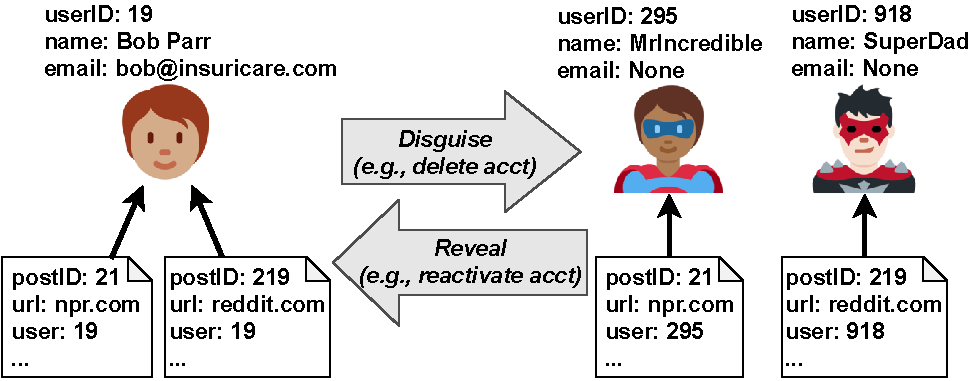
\includegraphics[width=0.5\textwidth]{img/disguises}

    \caption{Disguises move the target object (in this example, a user Bob) from an identity-revealing
    guise to privacy-preserving guises.}
    \label{fig:example}
\end{figure}
\fi

\begin{figure*}[t!]
    \centering
    \footnotesize
\begin{tabular}{@{}c|c|c|c@{}}
\textbf{User Transformation Spec} & \textbf{User Object} & \textbf{Guise 1} &
    \textbf{Guise 2} \\
\begin{lstlisting}[language=Rust]
"id":       IDAttribute,
"name":     Gen(Random),
"active":   Gen(Default(false)),
"darkmode": CopyAll,
"notifs":   CopyOnce+Gen(Default(false)),
"tag_id":   GenForeignKey,
\end{lstlisting}
    &
\begin{lstlisting}[language=Rust]
"id":       19,
"name":     BobParr,
"active":   true,
"darkmode": false,
"notifs":   true,
"tag_id":   11
\end{lstlisting}
&
\begin{lstlisting}[language=Rust]
"id":       295,
"name":     MrIncredible,
"active":   false,
"darkmode": false,
"notifs":   true,
"tag_id":   81483
\end{lstlisting}
&
\begin{lstlisting}[language=Rust]
"id":       918,
"name":     SuperDad,
"active":   false,
"darkmode": false,
"notifs":   false,
"tag_id":   15592
\end{lstlisting}
\end{tabular}
    \caption{Creating two guises of an example user (of a synthetic application schema).}
    \label{fig:guises}
\end{figure*}



The key idea behind \emph{data disguising} is to associate multiple \emph{guises} with a target
data object. Guises vary in how they reveal identities or preserve privacy.
%
Objects move between different guises by means of privacy transformations.
%
%Figure~\ref{fig:example} illustrates this with the example of user account deletion.
%
When his account is active, user Bob's profile is associated with his true identity and all his
contributions to the site (an identity-revealing guise).
%
When Bob deletes his account, his profile and contributions move to different, privacy-preserving
guises: his name has been anonymized, his email address has been redacted, and his contributions
have been decorrelated and attributed to individual, unidentified user guises.
%

%
Data disguising builds on the existing structure of web applications.
%
Web applications are often structured as object graphs, either explicitly~\cite{tao, delf},
through an object-relational model (ORM)~\cite{orm}, or implicitly via foreign keys (edges)
between tables (vertices) in relational databases.
%
Data disguises transform this object graph.
%

%
The application developer writes a disguise specification for each privacy transformation needed
in the application.
%
This specification is a declarative statement similar to a relational schema, with entries for
graph vertices (objects) and directed edges (relationships between pairs of objects)
to be transformed (see \S\ref{sec:policies}).
%
We assume that:
\begin{enumerate}[nosep]
  \item developers use their domain knowledge to write correct and complete disguises;
  \item application code handles the different guises appropriately (\eg in
    displaying them); and
  \item different guises of the same object have the same structure (\eg they can be
    rows in the same table).
\end{enumerate}
%
A data disguising tool takes the disguise specification and turns it into storage operations that
apply the transformation (disguise) or its reverse (reveal).
%
At any given moment, an application's data object graph comprises a mix of
identity-revealing guises and privacy-preserving ones. Privacy transformations split
and combine individual guises when triggered.

%-------------------------------------------------------------------------------
\section{Specifying Data Disguises}
%-------------------------------------------------------------------------------
\label{sec:policies}

A data disguise is written once by the developer, and applied in the context of a specific target
object to disguise, such as a departing user, and a specific instance of the object graph.
%
The disguise consists of context-specific transformations that turn objects into one or
more guises (or remove the object completely). Developers specify disguises in two parts. The
first specifies how to create guises of a given object type (\S\ref{sec:guises}). The second specifies in which
contexts objects should be transformed into guises or removed (\S\ref{sec:context}).

A disguising tool then applies the disguise by first determining the current context of objects in the object
graph, and then applying the appropriate transformation for that context.
%\ie from what type of edge, and sensitivity context.

\subsection{Creating Guises for Objects}
\label{sec:guises}
%
To create a guise from an object, developers specify how to transform attributes of the
object into guise attributes.
%
Figure~\ref{fig:guises} shows an example, producing guises for user objects.
%
User objects have identifier \texttt{id}; a reference \texttt{tag\_id}
forms an edge in the graph (a foreign key constraint to tag objects).

%
Guises always have unique, random identifiers.
%
Developers choose how to create other guise attributes, selecting from among the following:
%
\paragraph{(1) Copy object content.}
%
Guises of the same object all share the object's attribute values.
%
If the attribute is an edge attribute (\eg a foreign key column), all guises will have
edges to the same object.
%
%
Copying allows developers to retain the object's content, without worrying about how to
synthesize attribute values for guises.
%
For example, in Figure~\ref{fig:guises} the \texttt{darkmode} attribute is copied in
all guises.

\paragraph{(2) Generate new content.}
To create new attributes, developers specify whether the guise's value should be random,
a default value, or generated from the object's attribute value via a custom function (\eg hashing 
the value).
%
Figure~\ref{fig:guises} illustrates an example of random (\texttt{name}) and default
(\texttt{active}) generated value attributes.
%
%
Creating new guise edge attributes (\eg new foreign key relationships) requires
creating a new guise for the referenced object in order to maintain referential
integrity;
the data disguise rewrites the edge to point to the new guise.
%
In Figure~\ref{fig:guises}, creating two user guises requires creating two
tag guises, and the tag guises' identifiers become the user guises' foreign keys.
%

\paragraph{(3) Copy object content, but only once.}
%
One guise copies the attribute value from the object, but all other guises generate new
values (as described above).
%
\texttt{notifs} in Figure~\ref{fig:guises} illustrates how the attribute is copied once.
%
This enables the application to retain the original object semantics (\eg a count of how many
users want notifications) without creating duplicates.
%

\subsection{Context-Specific Transformations}
\label{sec:context}

Developers specify \emph{contexts} and the transformations to apply in each context.
%
% SOURCE = CHILD
% DEST = PARENT
%
In the following, we refer to edge types in the object graph, which have a \emph{source} object type and a \emph{destination} object type,
where the source references the destination (\eg via a foreign key column in a relational database).

Concretely, a context consists of:
\begin{enumerate}[nosep]
    \item A source object type
    \item A set of edge types from the source object type to different destination object types
    \item For each edge type: 
        \begin{itemize}[nosep]
            \item the transformation to perform on the edge type
            \item one or more constraints 
        \end{itemize}
\end{enumerate}

For any instance of the object graph, a set of objects and edges will satisfy the context if (1) the
objects are of the specified source object type; (2) the edges are of the specified edge types; and
(3) the edges satisfy the constraints on its edge type.

\vspace{\baselineskip}\noindent\textbf{Edge Type Transformations:}
\begin{enumerate}[nosep]
    %
    \item \textbf{Retain} edges of this type.
    %
    Transforms both source and destination objects into a single guise each.
    %
    \item \textbf{Decorrelate} the sources of edges of this type from their destination.
    %
    Creates one guise of the destination object for each of the sources; replaces each source's
    edge to the destination with an edge to that unique guise.
    %
    \item \textbf{Delete} the sources of edges of this type.
    %
    Transforms the destination object into a single guise; removes the source and its descendants.
    %
\end{enumerate}

\vspace{\baselineskip}\noindent\textbf{Edge Type Constraints:}
\begin{itemize}[nosep]
    \item A \textbf{threshold} constraint allows only some fraction of edges of a particular type to be
        transformed. 
        %decorrelation or deletion of edges to only partially occur. 
    %
    For example, Figure~\ref{fig:algo} illustrates a constraint that sets a threshold (0.5) for the
    maximum proportion of papers connected to a tag that a targer-user's papers can make up.
    Because the target user's papers make up more than 0.5 of all papers connected to the tag,
    \sys decorrelates the sensitive paper sources from the tag until the user's papers fall
    below or at the threshold.
    %
    If the threshold is negative, then \sys decorrelates or deletes \emph{all} sources of that
    destination, including sources that were not traversed from the target object.

\item A \textbf{directionality} constraint allows decorrelation to occur only for edges \sys traverses
    in the source-to-dest direction (step 2), or only for edges \sys traverses in the dest-to-source
    direction (step 3). This allows, for example, a paper that is co-authored by two users to
    decorrelate an edge to the target user, but retain an edge to the second, revealed author.
    %policies---higher sensitivity thresholds---allow \sys to retain links if \emph{only the
    %source} is sensitive, but decorrelate or remove the link if \emph{both} the source and dest
    %are sensitive. For example, perhaps a user wants to ensure that they are decorrelated from
    %their reviews, but correlations between the review and the the paper authors can still be
    %retained.

\item A \textbf{filter} constraint takes the edge's destination and source as inputs, and returns whether the objects satisfy the
    filter. 
    %
    For example, perhaps we want to decorrelate paper-tag edges
    \emph{only if} the tags were created by the user who is leaving.
\end{itemize}

\vspace{0.5\baselineskip}\noindent\textbf{Notes about Deletion.}
    Because of referential integrity, deleting an edge but keeping around the source object
    doesn't really make sense. The source needs a new destination to point to! I believe that
    decorrelation transformations capture what should happen if you want to ``delete the edge
    but keep the two nodes.'' Perhaps ``deletion edge transformation'' is a bad name because it
    implies that the edge (but maybe not the nodes) is removed.

    Directionality only matters for decorrelation: Deletion removes the source, and thus is unaffected by
    the direction of \sys's traversal, and retention is the same as a noop.

\subsection{An Example Disguise}
\label{design:eg}
%
Consider disguising Bob when he deletes his HotCRP account.
%
Bob would prefer his papers and reviews to be unlinked from his identity.
%
HotCRP, on the other hand, would like to retain paper and review information that other users
find useful.
%
A careful selection of edge and object transformations achieves both.
%

%
To decorrelate reviews from Bob, the disguise \texttt{Decorrelate}s user-to-review edges.
%
This requires transforming Bob into one unique user guise per review.
%
The disguise generates guise attribute values using suitable defaults;
%
in particular, HotCRP users' \texttt{disabled} attribute is set for the guises,
ensuring that guises have no permissions and never review papers.
%

%
Bob is further linked to papers through conflicts, which can indicate coauthorship or a
reviewer conflict.
%
These conflicts are not reassigned to the new guises, since preserved
conflicts could reidentify Bob as the likely author of a review. Thus, the
conflict edges that link a disguised user to papers need a \texttt{Delete} annotation.
%
%% Edge directionality matters here: paper-to-conflict edges should not be removed, as doing so
%% could incorrectly allow conflicted users to see the paper!

The disguise \texttt{Retain}s all other edge types, ensuring that review and paper
artifacts remain correctly linked. Active reviewers still see the correct paper for their reviews,
and active authors see the correct reviews for their papers, albeit potentially authored by
anonymous, unlinkable guises of the original reviewer.
%
%Review and paper guises copy the original object, retaining paper and review information.
%
%\ms{Does this mean duplicate papers/reviews can show up?}

%
Unlike the current real-world HotCRP account deletion policy~\cite{hotcrp:privacy}, which
deletes all objects belonging to Bob, this disguise strikes a balance between decorrelating
Bob's identity from his reviews and papers, and maintaining useful information for other
HotCRP users.
%
Furthermore, it is easy to imagine extending this disguise to automatically disguise Bob
after some time (\eg 2 years after the conference), protecting his future research career
by hiding youthful reviewing sins.
